\chapter{Развитие двумерной аксиально симметричной турбулентности}\label{ch:ch2}

\section{Вывод системы квазилинейных уравнений}\label{sec:ch2/sec1}

Поставленный вопрос и выяснение других качественных особенностей эволюции вейбелевской турбулентности, квазилинейных и не только, являются также актуальными для более реалистичной двумерной (2D3V) задачи, которая рассматривается в настоящем разделе и для которой расчеты кодом EPOCH являются более точными, поскольку его численные шумы не так сильно искажают функцию распределения частиц и динамику мод, как в одномерной задаче. Для определенности анализ ограничен простейшим аксиально симметричным случаем, в котором ось анизотропии $y$ исходного бимаксвелловского распределения электронов по скоростям (\ref{bimax}) ортогональна расчетной плоскости $xz$. В этом случае TEM-турбулентности, как будет ясно из дальнейшего, квазилинейные эффекты тоже доминируют и определяют основные свойства ее пространственного спектра. Последний для интересующих нас полей и токов представляется большим числом $s \cdot p$ неколлинеарных мод (гармоник) с волновыми векторами $\{ (k_{1}; k_{1}),\, (k_{1}; k_{2}),...,\, (k_{2}; k_{1}),...\, (k_{s}; k_{p}) \}$, компоненты которых состоят из $s$ радиальных проекций $\vec{k}\vec{r}_0$ и $p$ аксиальных проекций $\vec{k}\vec{\phi}_0$. В таком представлении обе компоненты магнитного поля, которое ортогонально оси анизотропии, имеют вид суммы мод по целочисленному векторному индексу $\vec{n}=(n_r,n_\phi)$:
\begin{align}
B_{x,z}(t,x,z) = \mathrm{Re} \sum^{l,p}_{n_r,n_\phi=1}\left(B_{k_{\vec{n}}}(t)\right)_{x,z}\exp(- \mathrm{i}\left(k_{\vec{n}}\right)_x x - \mathrm{i}\left(k_{\vec{n}}\right)_z z).
\end{align}
Аналогичен вид и единственной компоненты электрического поля $\vec{E}=(0, E_y, 0)$, направленного вдоль оси анизотропии функции распределения и ниже нормированного так же, как магнитное поле 
(\ref{eq19plus2}).

%систему (\ref{eq:f0.4})--(\ref{eq:maxw3.3}) с оператором (\ref{eq:oper.4})

Для указанных мод полей и возмущений-гармоник функции распределения электронов по скоростям получаем следующую систему квазилинейных уравнений с новым более сложным оператором $\hat \Theta_1$ вместо оператора $\hat \Phi$ одномерной задачи (ср. (\ref{eq:f0.3})--(\ref{eq:max_eq}), (\ref{eq:oper.2})): 
% \begin{wide}
\begin{align}
\label{eq:f0.4}
\dfrac{\partial \psi_0}{\partial \tau}+\sum\limits^{m}_{n=1}\mathrm{Re}\Bigg[\hat \Theta_1\left(e_{\vec{K}_{\vec{n}}},{\vec{b}}_{\vec{K}_{\vec{n}}},\psi_{K_n}^*\right)\Bigg]=0,\\
% \end{align}
% \begin{align}
\label{eq:f1.4}\dfrac{\partial \psi_{K_n}}{\partial \tau}+\mathrm{i}\left(K_{\vec{n}}\right)_x\beta_x\psi_{K_n}+\mathrm{i}\left(K_{\vec{n}}\right)_z\beta_z\psi_{K_n}+2\hat \Theta_1\left(e_{\vec{K}_{\vec{n}}},{\vec{b}}_{\vec{K}_{\vec{n}}},\psi_{0}\right)+\hat \Theta_1\left(e_{\vec{K}_{\vec{n}}}^*,{\vec{b}}_{\vec{K}_{\vec{n}}}^*,\psi_{2K_n}\right)=0,\\
% \end{align}
% \begin{align}
\label{eq:f2.4}
\dfrac{\partial \psi_{2K_n}}{\partial \tau}+2\mathrm{i}\left(K_{\vec{n}}\right)_x\beta_x\psi_{2K_n}+2\mathrm{i}\left(K_{\vec{n}}\right)_z\beta_z\psi_{2K_n}+\hat \Theta_1\left(e_{\vec{K}_{\vec{n}}},{\vec{b}}_{\vec{K}_{\vec{n}}},\psi_{K_n}\right)=0,\\
% \end{align}
% \begin{align}   
    \dfrac{\partial \left({b}_{\vec{K}_{\vec{n}}}\right)_z}{\partial \tau}=-\mathrm{i}\left(K_{\vec{n}}\right)_xe_{\vec{K}_{\vec{n}}},\quad 
    \dfrac{\partial \left({b}_{\vec{K}_{\vec{n}}}\right)_x}{\partial \tau}=\mathrm{i}\left(K_{\vec{n}}\right)_ze_{\vec{K}_{\vec{n}}}, \\
\label{eq:maxw3.3}
    \dfrac{\partial e_{\vec{K}_{\vec{n}}}}{\partial \tau}=\mathrm{i}\left({b}_{\vec{K}_{\vec{n}}}\right)_x\left(K_{\vec{n}}\right)_z-\mathrm{i}\left({b}_{\vec{K}_{\vec{n}}}\right)_z\left(K_{\vec{n}}\right)_x+\beta_{\|0}^{-1}{\iiint\limits^{+\infty}_{-\infty}\beta_y\psi_{\vec{K}_{\vec{n}}}(\tau,\beta_x,\beta_y,\beta_z)d\beta_xd\beta_yd\beta_z} ,\\
% \end{align}
% \begin{align}
\label{eq:oper.4}
\hat \Theta_1\left(e_{\vec{K}_{\vec{n}}},{\vec{b}}_{\vec{K}_{\vec{n}}},\psi(\beta)\right)  =  \dfrac{e_{\vec{K}_{\vec{n}}}}{2}\dfrac{\partial \psi(\beta)}{\partial \beta_y}-\dfrac{\left({b}_{\vec{K}_{\vec{n}}}\right)_z}{2} \left(\beta_x\dfrac{\partial \psi(\beta)}{\partial \beta_y}-\beta_y\dfrac{\partial \psi(\beta)}{\partial \beta_x}\right) \nonumber \\
-\dfrac{\left({b}_{\vec{K}_{\vec{n}}}\right)_x}{2} \left(\beta_z\dfrac{\partial \psi(\beta)}{\partial \beta_x}-\beta_x\dfrac{\partial \psi(\beta)}{\partial \beta_z}\right) .
\end{align}
% \end{wide}


\section{Сравнение с результатами моделирования методом частиц в ячейках. Выявление нелинейных эффектов четырехволнового взаимодействия на фоне квазилинейной динамики мод.}\label{sec:ch2/sec1}
Мы исследовали ее двумерно-неоднородные решения, получаемые численно на основе метода Стёрмера~-- Верле (Leapfrog)~\cite{Birdsall2018} (см. конец раздела 2) при одной и той же исходной поперечной тепловой скорости $\beta_{\perp0}=0.1$ и различной начальной анизотропии. Кроме того, опять проводилось сравнение с моделированием методом частиц в ячейках при помощи кода EPOCH, которое в целом оказалось согласованным с квазилинейным моделированием системы (\ref{eq:f0.4})-(\ref{eq:oper.4}) с точностью $\sim10-30\%$. Соответствующие результаты приведены ниже при $A_0=0.25$ и $A_0=10$, как и в предыдущем разделе для одномерной задачи. Отметим, что и для двумерной задачи в предположении об аксиально симметричном и достаточно узком пространственном спектре вейбелевской турбулентности, согласно~\cite{Nechaev2023} и (\ref{eq:otsenka}), нетрудно получить следующее приближенное аналитическое соотношение для эволюционирующих среднеквадратичного магнитного поля $b_{av}$, параметра анизотропии плазмы $A$ (ср. (\ref{eq:A_1d})) и среднего радиального волнового числа (\ref{eq:angles}) $\langle K\rangle$ (ср. начало раздела 3): 
\begin{equation}
\label{eq:otsenka2d}
b_{av}^2 = \frac{A_0-A}{1+A_0}\cdot\dfrac{\langle K\rangle^2}{A \langle K\rangle^2+A+5\langle K\rangle^2+3} ,
\end{equation}
\begin{equation}
\label{eq:A_2d}
A=\frac{2\iiint\limits^{\infty}_{-\infty}\beta_y^2\psi_{0}(\tau,\beta_x,\beta_y,\beta_z) d\beta_x d\beta_yd\beta_y}{\iiint\limits^{\infty}_{-\infty}\left(\beta_x^2+\beta_z^2\right)\psi_{0}(\tau,\beta_x,\beta_y,\beta_z) d\beta_x d\beta_y d\beta_z}-1 .
\end{equation}
Это соотношение для аксиально симметричной (в среднем) турбулентности по-прежнему очень хорошо, с точностью до нескольких процентов, выполнялось в квазилинейных расчетах~(см., например, рис.~\ref{fig:evol2d}a) и немного хуже, с точностью до 10-20\%, в расчетах методом частиц в ячейках, где в условиях высокого уровня численных шумов спектр оказывался более широким. Отметим, что всюду ниже под спектром вейбелевской турбулентности в аксиально симметричной задаче подразумевается зависимость нормированных амплитуд мод магнитного поля (\ref{eq19plus1}) $|b_K|$ от нормированного радиального волнового числа (\ref{eq19plus2}) $K$, получаемая после усреднения по азимутальному углу. 
\begin{figure}[t]
\centering
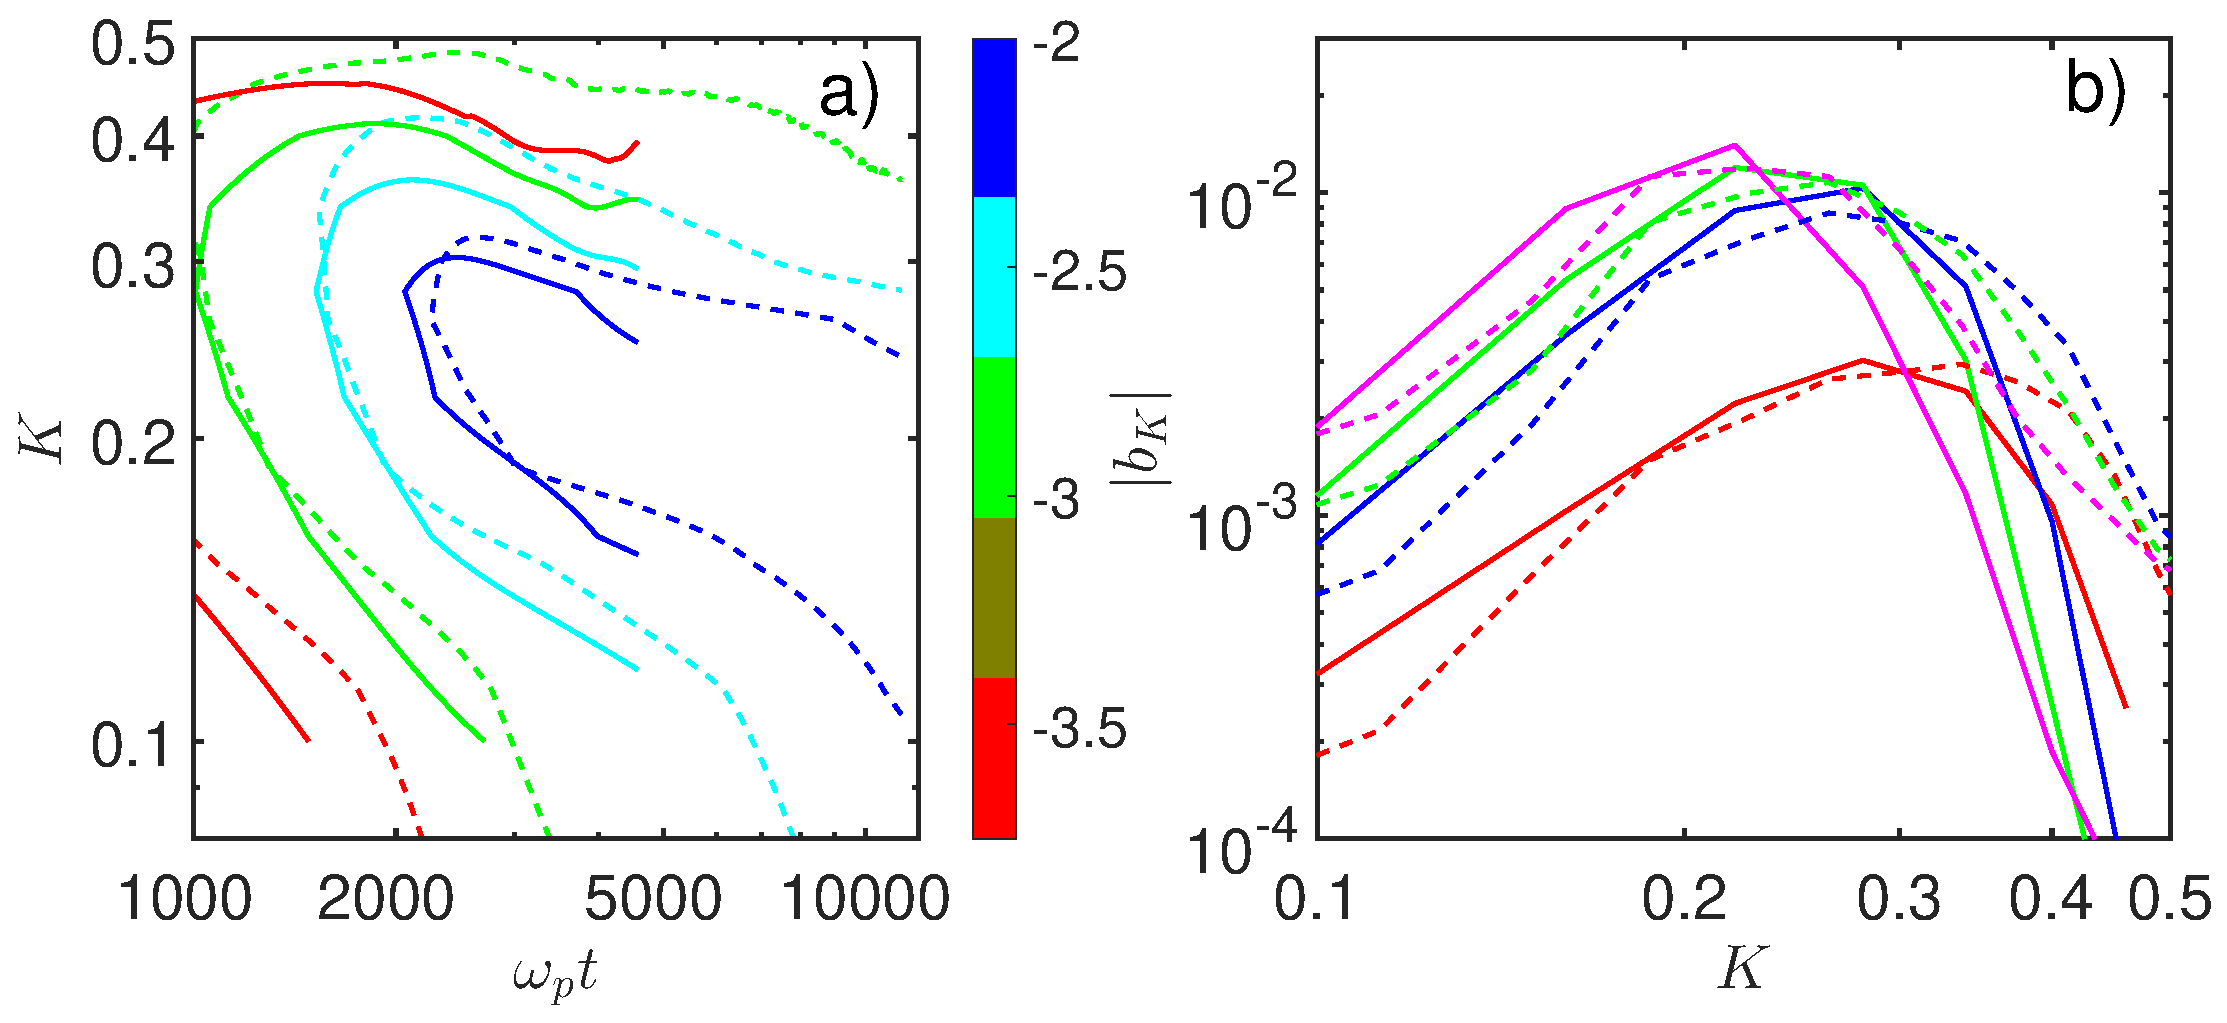
\includegraphics[width=0.9\linewidth]{part2/fig13.eps}
\caption{Эволюция спектра турбулентности, найденная в аксиально симметричных расчетах методом частиц в ячейках (штрихи) и на основе квазилинейного подхода (сплошная линия), в двойном логарифмическом масштабе: (a)~линии уровня логарифма амплитуд мод магнитного поля $|b_K|$; (b)~спектр $|b_K|$ магнитного поля в моменты времени $\wpl t$, равные 1500 (красный цвет), 2400 (синий), 3000 (зеленый) и 4500 (розовый). Начальная анизотропия $A_0=0.25$.
}
\label{fig:dinspectrA025_2d}
\end{figure}


Не повторяя общие положения, сформулированные в подразделах 3.1 и 3.2, сосредоточимся только на различиях в развитии турбулентности, обусловленных переходом от одномерной к двумерной задаче, т.\,е. расширением области волновых векторов неустойчивых мод и направлений их магнитных полей, а следовательно, усилением квазилинейного взаимодействия мод и деформации функции распределения электронов по скоростям.
\begin{figure}[t]
\centering
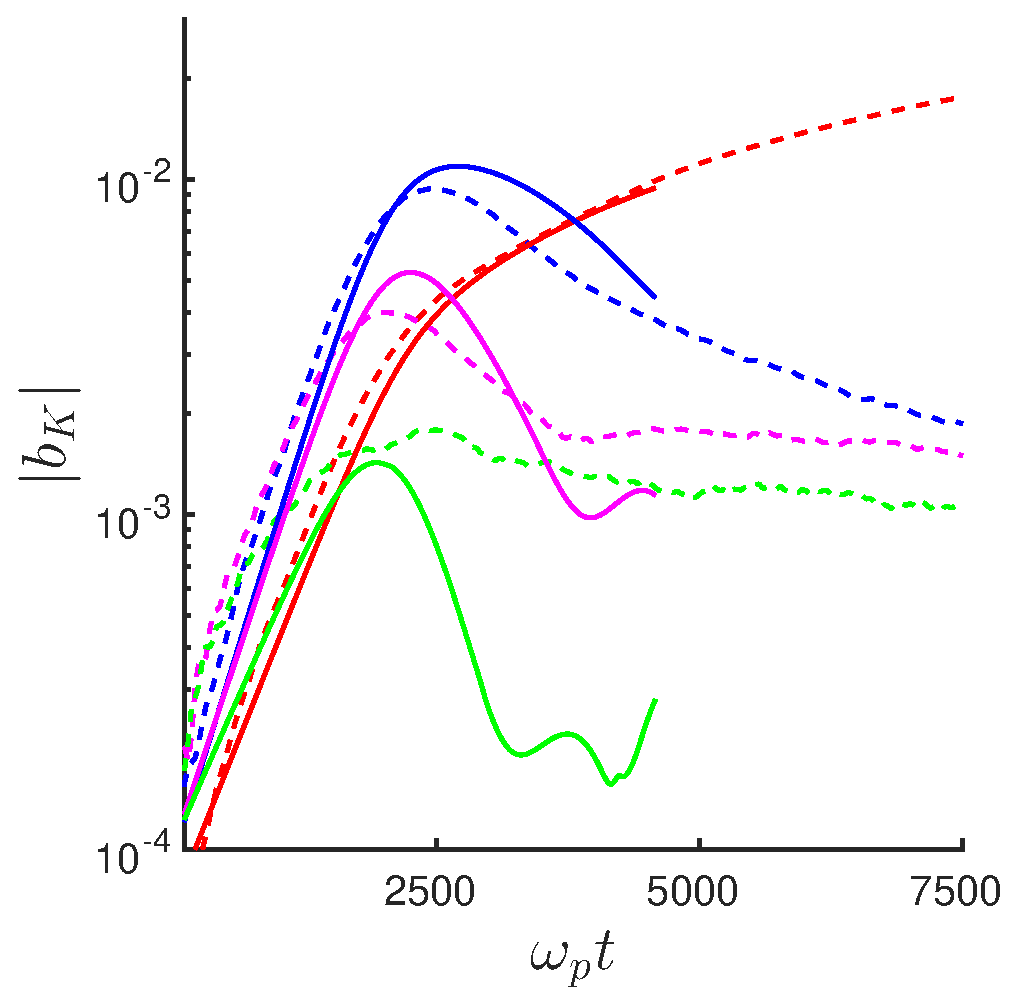
\includegraphics[width=0.5\linewidth]{part2/fig14.eps}
\caption{Эволюция четырех типичных мод ($K=0.16$ --- красный цвет, $K=0.28$ --- синий, $K=0.34$ --- розовый, $K=0.4$ --- зелёный), взятых из спектра рис. \ref{fig:dinspectrA025_2d}. Оптимальное волновое число $K_\mathrm{opt}\approx0.28$.}
\label{fig:evol_garmA025}
\end{figure}

При низкой начальной анизотропии, $A_0=0.25$, деформация функции распределения идет интенсивнее, дольше и по величине составляет уже не доли, а несколько процентов, захватывая более обширную область тепловых скоростей электронов, так что тангенс угла конуса, на котором согласно рис.~\ref{fig:sravnenie_FR1d} меняется знак приращения функции распределения, увеличивается от примерно 1/6 до почти 1/2. При этом в баунс-осцилляциях участвует больше электронов, а функция распределения становится менее анизотропной и по форме ближе к бимаксвелловской, причем величина анизотропии с наступлением нелинейной стадии падает не осциллируя и не на 1-2\% (как было показано на рис.~\ref{fig:evol1d_QL_A025}b), а почти на 20\%, продолжая снижаться в дальнейшем. Значительнее уменьшается, не осциллируя, и среднее волновое число $\langle K\rangle$ энергонесущих мод, а насыщающее среднеквадратичное магнитное поле $b_{sat}$ оказывается сильнее приблизительно в 5 раз и тоже не осциллирует, хотя по-прежнему почти не снижается по величине на рассмотренных временах, в несколько раз превышающих время наступления насыщения. Данные результаты квазилинейного подхода согласуются с предшествующими численными исследованиям вейбелевской неустойчивости методом частиц в ячейках, например,~\cite{Borodachev2010,Borodachev2016_Radiofiz}. 

В рассмотренном типичном примере смещение спектра турбулентности в длинноволновую область, как показано на рис.~\ref{fig:dinspectrA025_2d}, выражено более явно и сопровождается затуханием коротковолновых мод, а не только ростом длинноволновых, что имело место в одномерной задаче (ср. рис.~\ref{fig:dinspectrA025_1d}, где время наступления насыщения почти вдвое больше, поскольку логарифмический уровень начальных амплитуд мод был задан примерно вдвое ниже, чем на рис.~\ref{fig:dinspectrA025_2d}). Такое поведение спектра обусловлено более эффективным квазилинейным, но не четырехволновым взаимодействием мод, что подтверждает аналогичный расчет методом частиц в ячейках, который учитывает оба механизма взаимодействия мод и которому на рисунке отвечают штриховые линии, хорошо совпадающие со сплошными. Благодаря менее анизотропной и более гладкой форме функции распределения, согласованной с двумерной турбулентностью, отдельные моды в ходе ее эволюции остаются по существу апериодическими, т.\,е. их инкременты (декременты) превышают по величине возможные значения действительных частот. Следовательно, в отличие от одномерной турбулентности, квазипериодические осцилляции амплитуд мод практически отсутствуют и их начальный рост с последующим затуханием определяется изменяющейся величиной инкремента, переходящего после насыщения в декремент; ср. рис. \ref{fig:evol_garmA025} и \ref{fig:evol_garmA025_1d}. При этом из-за изменения во времени инкремента (декремента) мод оказывается возможным не строго экспоненциальный, а скорее близкий к степенному как рост их амплитуд на промежуточном этапе эволюции до достижения максимальной величины (который начинается после насыщения наиболее быстро растущей моды с оптимальным волновым числом $K_\mathrm{opt}\approx0.28$), так и дальнейшее затухание. Со временем совместная динамика мод отражается в автомодельных чертах спектра турбулентности $|b_K|$, у которого в представленном примере длинноволновое и коротковолновое крылья неплохо аппроксимируются степенными зависимостями с показателями около 2 и -10 соответственно.
\begin{figure}[t]   
\centering
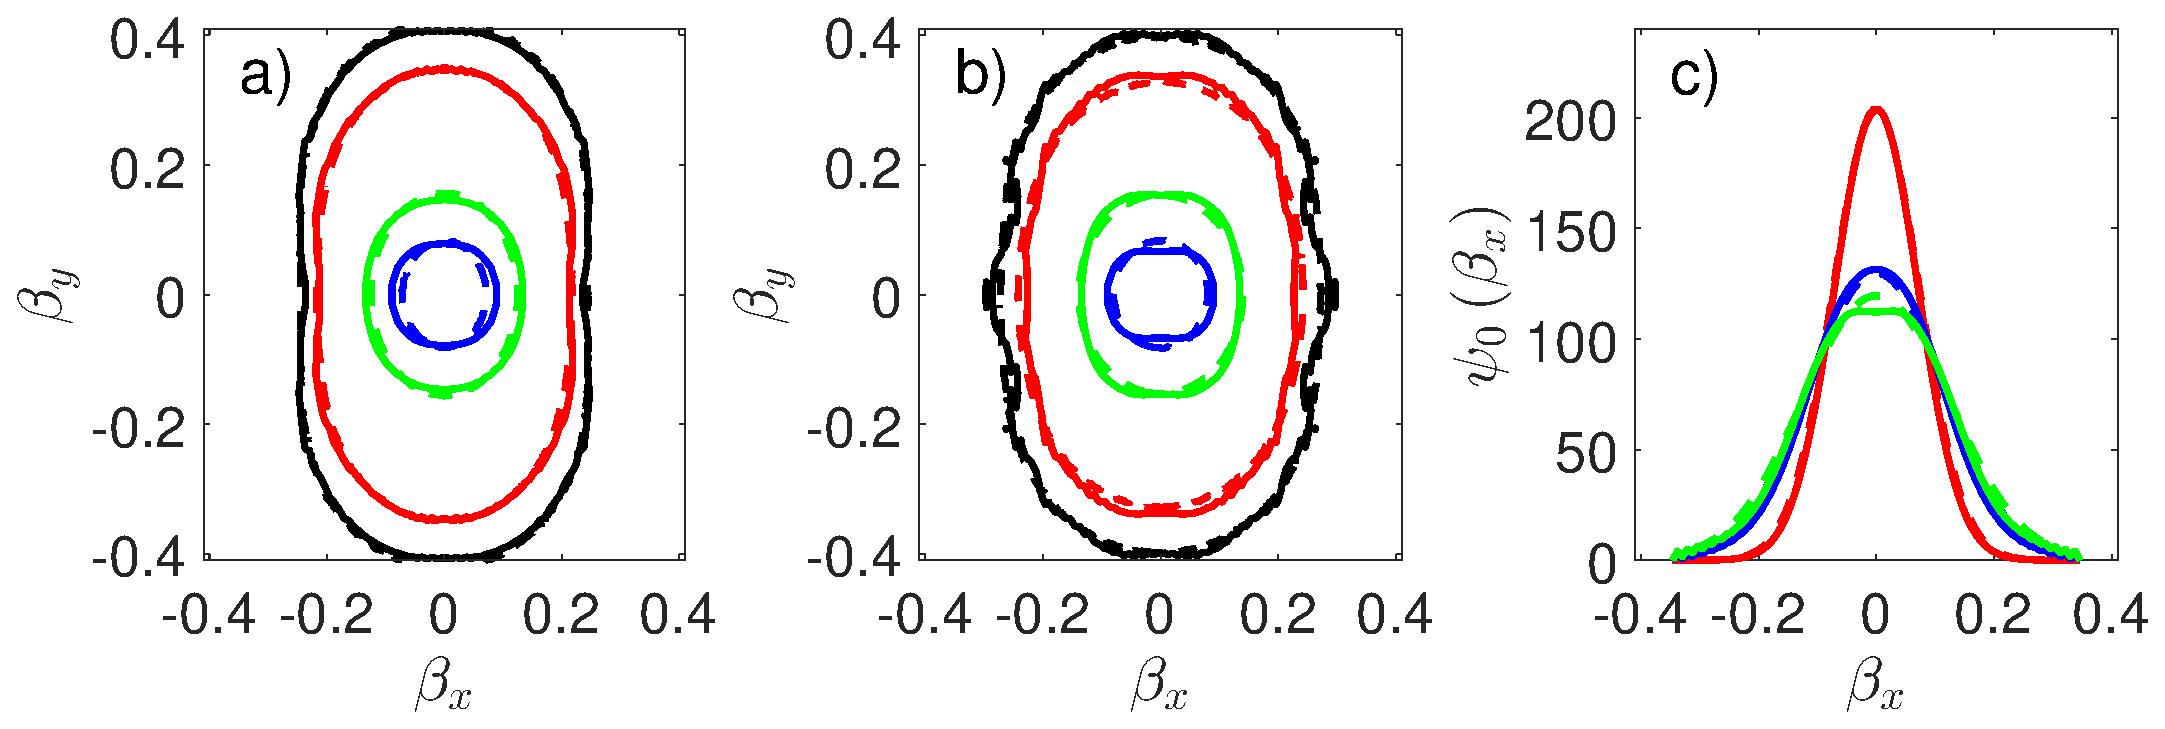
\includegraphics[width=0.9\linewidth]{part2/fig15.eps}
\caption{(a)~Линии уровня $0.05$ (черный цвет), $0.1$ (красный), $0.5$ (зелёный) и $0.8$ (синий), отсчитанные от максимального значения функции распределения в момент времени $\wpl t =83$; (b)~то же в момент времени $\wpl t =170$; (c)~распределение частиц по величине нормированной компоненты скорости $\beta_x$, ортогональной оси анизотропии, в моменты времени $\wpl t$, равные 0 (красный цвет), 83 (синий) и 170 (зеленый). Приведены данные аксиально симметричных расчетов методом частиц в ячейках (штрихи) и в рамках квазилинейного подхода (сплошная) при $A_0=10$.
}
\label{fig:sravnenie_FR2dax_3im}
\end{figure}

\begin{figure}[b]
\centering
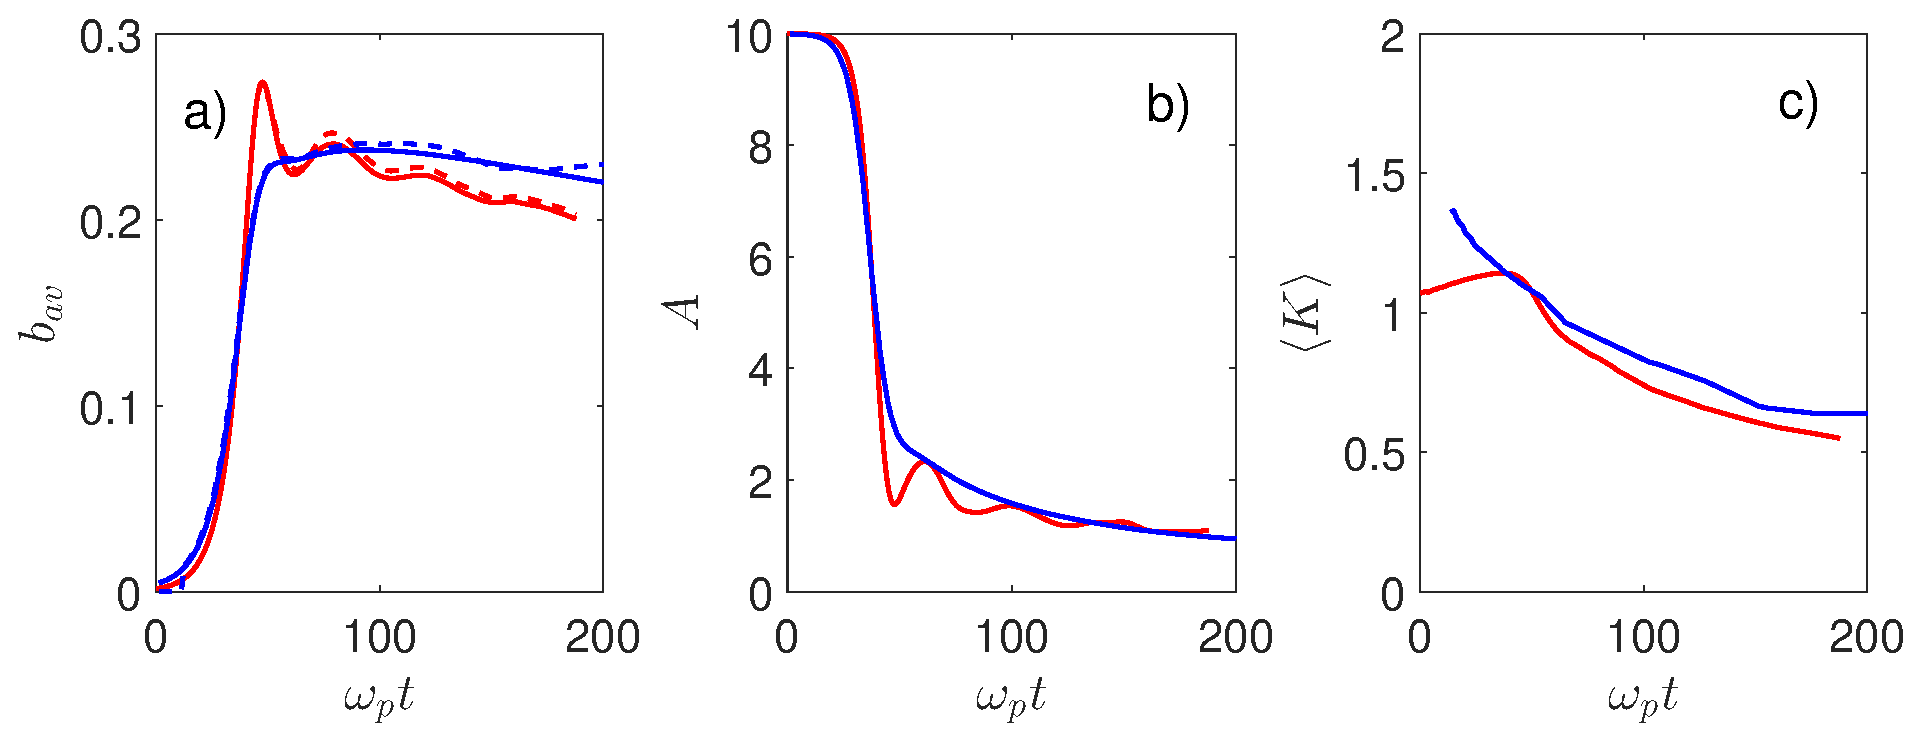
\includegraphics[width=1\linewidth]{part2/fig16.eps}
\caption{Эволюция (a) среднеквадратичного магнитного поля $b_{av}$ (сплошная линия) и оценки этой величины~(\ref{eq:otsenka2d})~(штрихи), а также (b) параметра анизотропии $A$ и (c) характерного волнового числа $\langle K\rangle$ согласно численному квазилинейному моделированию (красный цвет) и расчетам методом частиц в ячейках (синий цвет) в аксиально симметричной задаче при $A_0=10$.}
\label{fig:evol2d}
\end{figure}
Остановимся теперь на ситуации с высокой начальной анизотропией, $A_0=10$, опять опираясь на во многом идентичные результаты расчетов с использованием квазилинейного подхода и метода частиц в ячейках. Как показывает сравнение рис. \ref{fig:sravnenie_FR2dax_3im} и \ref{fig:sravnenie_FR1d_A10}, не только качественное, но и количественное отличие деформаций функции распределения электронов по скоростям в одномерной и двумерной задачах не очень велико. Впрочем, в последней линии уровня этой функции являются более овальными, менее прямоугольными, что соответствует более сглаженной, менее анизотропной форме, хотя все равно значительно отличной от бимаксвелловской во всей области скоростей порядка тепловых. При этом падение параметра анизотропии $A$ в процессе насыщения неустойчивости происходит немного плавнее, но и немного глубже, так что насыщающее магнитное поле $b_{av}$ тоже оказывается немного выше и после резкого нарастания очень медленно затухает, слегка осциллируя в противофазе с анизотропией на величину порядка нескольких процентов; ср. рис. \ref{fig:evol1d_QL_A10} и \ref{fig:evol2d}. 

Согласно рис. \ref{fig:dinspectrA10_1d} и \ref{fig:dinspectrA10_2d}, эволюция одномерного и двумерного спектра вейбелевской турбулентности в целом однотипна, а волновое число, отвечающее его максимуму (и почти совпадающее со средним значением $\langle K\rangle$), смещается в длинноволновую сторону примерно по одному и тому же степенному закону $t^{-1/2}$ (см. также рис. \ref{fig:evol2d}c; этот закон отмечался нами ранее~\cite{Borodachev2016_Radiofiz,Nechaev2019_Radiophys}). Важным, однако, представляется выявление следующих отличий в спектре двумерной турбулентности, вычисленном в квазилинейном подходе и с помощью кода EPOCH при высокой начальной анизотропии $A_0=10$. Именно, с началом стадии насыщения, $\wpl t > 60$, в коротковолновой части спектра, $K > K_\mathrm{opt}$, квазилинейный расчет демонстрирует осцилляторное поведение мод, тогда как оно отсутствует в аналогичном расчете методом частиц в ячейках, демонстрирующем резкое и существенное, по меньшей мере двукратное, расширение спектра в коротковолновую сторону. Этих отличий не было при низкой начальной анизотропии $A_0=0.25$, а также в одномерной турбулентности ни при какой начальной анизотропии. Указанное расширение спектра особенно наглядно видно на рис. \ref{fig:dinspectrA10_2d}b на больших временах $\wpl t =$ 160 и 280, когда квазилинейный расчет (сплошные кривые) показывает сильное смещение крутого правого крыла спектра в длинноволновую сторону, а более точный расчет кодом EPOCH (штрихи) сохраняет правое крыло гораздо более коротковолновым и пологим. Отметим, кстати, что соответствующие степенные показатели -3.5 и 3 правого и левого крыльев спектра двумерной турбулентности сильно отличаются от аналогичных показателей -10 и 2 спектра одномерной турбулентности при той же величине $A_0=10$, что отчасти связано с разным уровнем заданных начальных амплитуд мод. 



\begin{figure}[t]
\centering
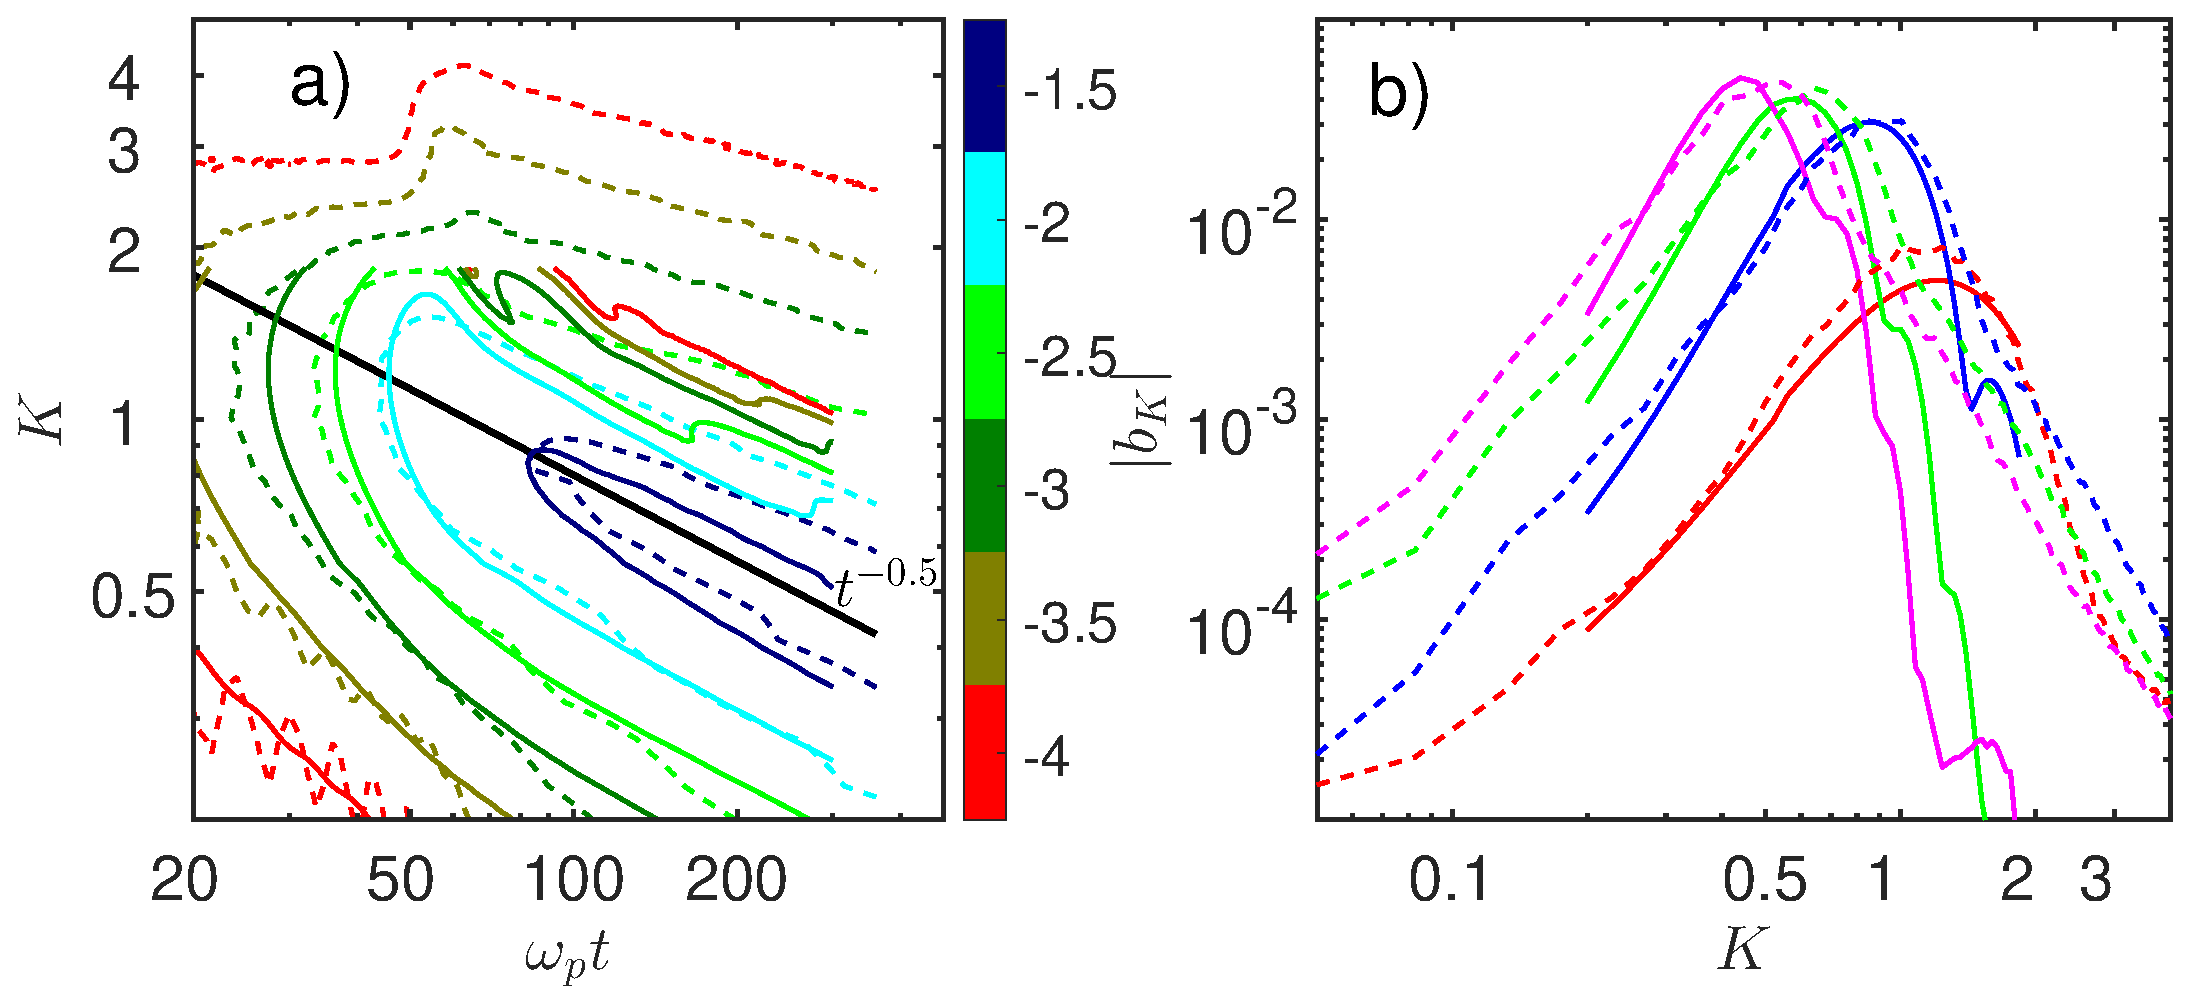
\includegraphics[width=0.9\linewidth]{part2/fig17.eps}
\caption{Эволюция спектра турбулентности, найденная в аксиально симметричных расчетах методом частиц в ячейках (штрихи) и в рамках квазилинейного подхода (сплошная линия), в двойном логарифмическом масштабе: (a)~линии уровня логарифма амплитуд мод магнитного поля $|b_K|$; 
(b)~спектр $|b_K|$ магнитного поля в моменты времени $\wpl t$, равные 40 (красный цвет), 80 (синий), 160 (зеленый) и 280 (розовый). Начальная анизотропия $A_0=10$.
}
\label{fig:dinspectrA10_2d}
\end{figure}
Причина установленных отличий, скорее всего, заключается в четырехволновом взаимодействии мод, не учитывающимся в квазилинейной системе уравнений (\ref{eq:f0.4})-(\ref{eq:oper.4}). Последняя благодаря этому обстоятельству позволяет выявить в моделировании методом частиц в ячейках нелинейные эффекты, отличные от квазилинейных. Сравнение расчетов одной и той же задачи в рамках этих двух подходов полезно провести путем анализа динамики отдельных мод двумерной вейбелевской турбулентности с использованием рис.~\ref{fig:evol_garm}. Расчет кодом EPOCH (штрихи) показывает, что с наступлением насыщения турбулентности достаточно коротковолновые моды, вопреки квазилинейному приближению (сплошные линии), не следуют осцилляторной динамике и экспоненциальному затуханию с легко вычисляемыми показателями порядка 0.01 - 0.1 (что примерно вдвое больше, чем для аналогичной одномерной турбулентности; ср. рис.~\ref{fig:evol_garmA010_1d}). Напротив, эти моды лишь частично, в небольшой мере отслеживают первую <<квазилинейную>> осцилляцию и довольно быстро переходят к медленному примерно степенному затуханию с показателями в небольшом интервале значений от -1 до -1.3, по-видимому, испытывая эффективную подкачку за счет четырехволнового взаимодействия немного более длинноволновых мод, имеющих достаточно большие амплитуды и расположенных в центральной части текущего спектра. 

\begin{figure}[b]
\centering
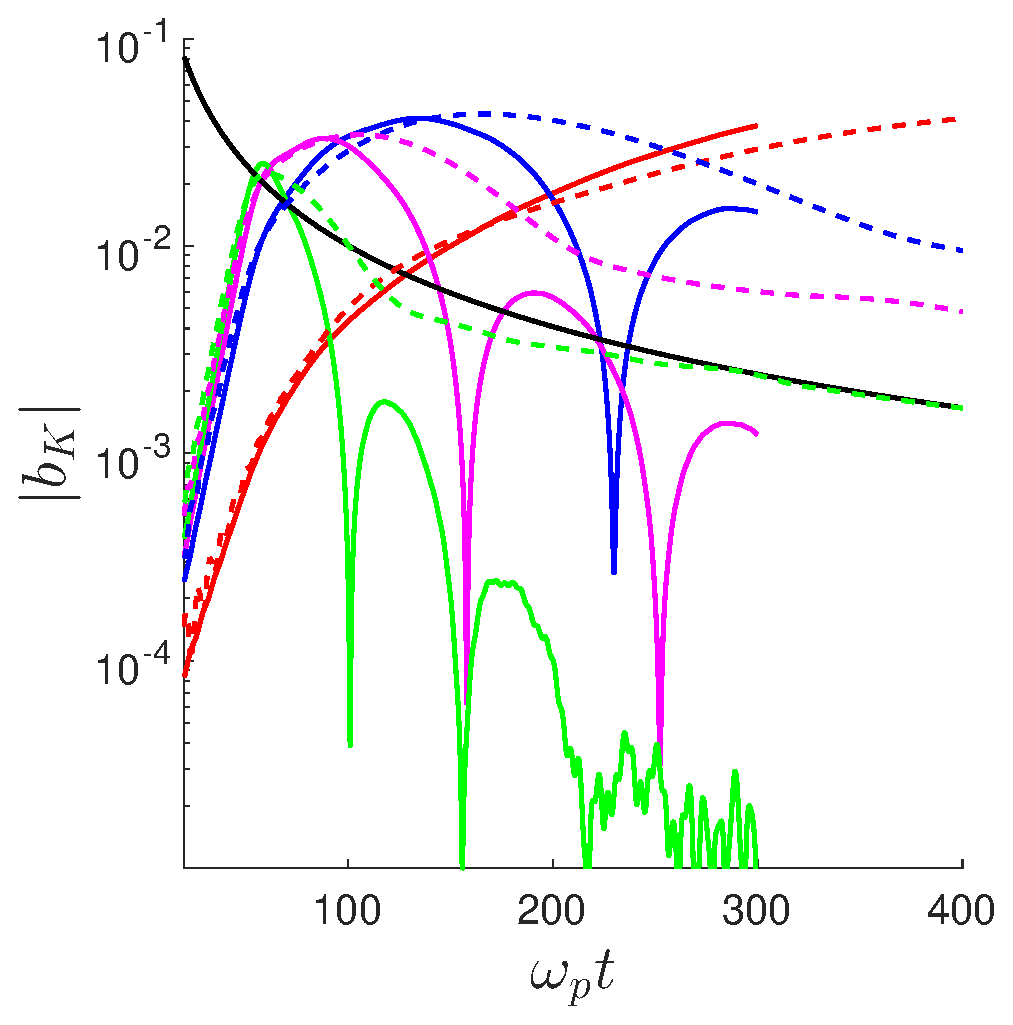
\includegraphics[width=0.5\linewidth]{part2/fig18.eps}
\caption{Эволюция четырех типичных мод ($K=0.36$ --- красный цвет, $K=0.68$ --- синий, $K=0.88$ --- розовый, $K=1.2$ --- зелёный), взятых из спектра рис. \ref{fig:dinspectrA10_2d}. Оптимальное волновое число $K_\mathrm{opt}\approx1.2$. Черная линия соответствует степенной зависимости $t^{-4/3}$.}
\label{fig:evol_garm}
\end{figure}
Вместе с тем, значительно более длинноволновые моды находятся, вплоть до своего насыщения, на промежуточной стадии приблизительно степенного роста с показателями порядка 1 - 2 (что в два-три раза меньше, чем для аналогичной одномерной турбулентности). Подобная динамика этих мод может объясняться квазилинейным образом при надлежащей зависимости от времени их инкрементов, но может быть обусловлена, хотя бы частично, все той же нелинейной подкачкой при четырехволновом взаимодействии более мощных мод из центральной части спектра турбулентности. Не исключено также, что еще более длинноволновые моды, которые только выходят или не далеко отошли от уровня шумов на стадии насыщения турбулентности, могут быть сильно, даже сверхэкспоненциально, возбуждены нелинейным образом посредством четырехволнового взаимодействия с какими-либо более мощными модами, что в результате может влиять на форму длинноволнового крыла спектра турбулентности. Данный круг вопросов требует дальнейшего детального исследования. 

Во избежание недоразумений следует отметить, что вплоть до насыщения роста среднеквадратичного магнитного поля отличия квазилинейных расчетов от расчетов методом частиц в ячейках являются весьма незначительными, даже в одномерной задаче. В итоге, квазилинейный подход позволяет корректно вычислять величину насыщающего магнитного поля вейбелевской турбулентности, что уже было продемонстрировано в конце подраздела 3.1 на рис.~\ref{fig:bsat}. Согласно ему, средний квадрат насыщающего поля двумерной турбулентности отличается от его значения для одномерной на десятки процентов при большом начальном параметре анизотропии, $A_0\gtrsim1$, и многократно при низком параметре, $A_0\lesssim1$, поскольку тогда численно найденный показатель его степенной зависимости от этого параметра оказывается близким к 2 вместо аналитически найденного показателя 5 для одномерной турбулентности (см. формулу (\ref{eq:analit_estimation})). 

Таким образом, проведенные расчеты, в том числе и для других параметров анизотропии $A_0$, показывают следующие существенные различия эволюции спектра вейбелевской турбулентности в одномерной и аксиально симметричной двумерной задачах при одинаковых начальных условиях. 

Во-первых, более богатый двумерный спектр развитых мод обеспечивает более гладкую и сильную модификацию исходной функции распределения электронов по скоростям, а следовательно, более значительные уменьшение параметра анизотропии и увеличение магнитной энергии турбулентности. При этом последующий распад образовавшихся случайных самосогласованных токовых филаментов идет эффективнее, чем для турбулентности с одномерным спектром, где квазилинейные эффекты и четырехволновое взаимодействие мод искусственно ограничены, как и свободный разлет электронов из токовых слоев.

Во-вторых, в двумерном случае автомодельный характер эволюции спектра выражен более явно, а формирование его степенных крыльев и смещение его максимума в длинноволновую сторону происходят быстрее, возможно, благодаря не только квазилинейному, но и четырехволновому взаимодействию мод. При этом зависимость соответствующих параметров спектра от начальной анизотропии плазмы выражена слабее, чем в одномерном случае, где перестройка спектра заторможена.

В-третьих, динамика отдельных мод в двумерной задаче, естественно, оказывается более сложной и многообразной, хотя в общем случае и включает в себя те же три основные стадии, что и в одномерной задаче: сначала экспоненциальное и потом примерно степенное нарастание, а после достижения максимума -  тоже спадание степенного типа. При этом в одномерной турбулентности для многих мод не все эти стадии четко выражены, но значительно заметнее квазипериодические осцилляции амплитуд мод и даже ее интегральных характеристик, вызванные, как и в двумерной турбулентности, квазилинейной модификацией анизотропии функции распределения электронов и соответствующим изменением действительных частот и инкрементов (декрементов) мод.
  